\chapter{Event Reconstruction and Selection}
The data from the HPS detector must be reconstructed and calibrated before it can be used in an analysis.
Furthermore, the contents of the data must be understood and shown to be consistent with known physics before we can trust it in a search for new physics.
This chapter describes that process.

\section{Reconstruction}
The HPS event reconstruction is based on the org.lcsim software toolkit \cite{graf_org.lcsim:_2011}.
The basic outputs of the event reconstruction are tracks in the SVT and clusters in the ECal.
The reconstruction also matches clusters to tracks, and fits pairs of charged tracks to vertices.

The HPS coordinate system used in reconstruction is defined by the Hall B beamline.
The Z-axis points downstream along the Hall B axis, in the direction the beam takes before it reaches the HPS chicane.
The Y-axis points up, and coincides with the magnetic field direction.
The X-axis points to beam-left, in the bend plane.
The origin is set at the intersection of the beam with the nominal target position.

Because the target is not in the center of the chicane, the HPS beam axis (the direction of the beam when it intersects the target) is rotated by 30.5 milliradians relative to the Z-axis.
The reconstructed momenta of particles at the target are distributed symmetrically around the HPS beam axis, not the Hall B axis.
Since the HPS beam axis is the natural reference frame for reconstructed particles, reconstructed momenta and vertex positions are typically rotated by 30.5 milliradians to put them in the HPS beam frame.

\subsection{Tracking}
\label{sec:track_recon}
A charged particle track in a uniform field follows a helix.
HPS uses the ``perigee'' parametrization for tracks, where the track position and direction are defined at the point of closest approach to the origin (the perigee) in the X-Z frame.
The standard definition of the perigee parametrization fixes the magnetic field along the Z-axis; this is not the case for HPS, but we retain the standard parameter names (e.g. $z_0$).
The curvature is defined as $C=-q/R$, where $q$ is the charge and $R$ is the helix radius; it is proportional to $1/p_\perp$, where $p_\perp$ is the component of momentum that is perpendicular to the magnetic field.
The track position is defined by the distance of closest approach in the X-Z frame $d_0$, and the height at closest approach $z_0$.
The track direction is defined by the angle from the Z-axis at closest approach $\phi_0$, and the slope at closest approach $\tan\lambda$.

For HPS tracks, the point of closest approach to the origin is always near the origin, and the track direction there is always close to the Z-axis.
This means that $d_0$ and $z_0$ can be interpreted (approximately) as the track $x$ and $y$ at $z=0$, and $\phi_0$ and $\tan\lambda$ are approximately equal to $\theta_x$ (the angle of elevation from the Y-Z plane) and $\theta_y$ (the angle of elevation from the X-Z plane).

Multiple scattering in the silicon sensors means that different segments of the track may be described by different helices.
A full HPS track fit (after GBL refit, as described in Section \ref{sec:track_finding_refit}) has a different helix before and after every sensor: a track with hits on 12 sensors has 13 track segments.
The track segment of interest for the analysis is the one at the target (before the first sensor), and this is what is used unless otherwise specified.

\subsubsection{Hit Reconstruction}
\label{sec:svt_hit_recon}
For each strip above threshold, the SVT readout stores a waveform of six samples at 24 ns intervals.
The readout is aligned with the trigger such that typically, two or three of the samples are taken before the trigger, and three or four samples are taken after the trigger.
This is enough points to both fit a pulse that is in time with the trigger, and a pileup pulse that may arrive before or after the trigger.

The APV25 response is modeled as a filter with four poles, three of them coincident.
This is the transfer function, where $\tau_1\approx 72$ ns and $\tau_2\approx 12$ ns are the two time constants:
\begin{equation}
    \tilde{F}_{4pole}(\omega) = \frac{1}{(1+j\omega\tau_1)(1+j\omega\tau_2)^3}
\end{equation}
The pulse shape is the impulse response, which is the inverse Fourier transform of the transfer function.
With $t$ defined as the time after the start of the pulse, the impulse response is as follows:
\begin{equation}
    F_{4pole}(t) = \frac{\tau_1^2}{(\tau_1-\tau_2)^3} \left( e^{-\frac{t}{\tau_1}} - e^{-\frac{t}{\tau_2}} \sum_{k=0}^3 \frac{\left(\frac{\tau_1-\tau_2}{\tau_1\tau_2}t\right)^k}{k!} \right)
\end{equation}

The pulse fitting algorithm attempts two different fits: a fit to a single pulse with unknown time and amplitude, and a fit to the sum of two pulses with different times and amplitudes.
The $\chi^2$ of the two fits are compared to decide whether the waveform is better fit by a single pulse or two pulses.
The pedestal and the shaping times $\tau_1$ and $\tau_2$ are calibrated offline.
It is possible to fit the pedestal on an event-by-event basis to better handle an effect where the pedestal shifts in high-occupancy channels; this part of the algorithm was not active for this analysis.

After pulse fitting, each strip above threshold in the SVT has one or two hits, with times (relative to the trigger) and amplitudes (in units of ADC counts).
It is not crucial to express the hit amplitudes in terms of energy deposition, and gains in different channels do not vary by enough to affect the reconstruction, so amplitudes are left in terms of ADC counts even though gain information is available from calibrations.

Fitted hits are merged to form clusters if they appear to be from the same particle.
The position of a cluster is the amplitude-weighted centroid ($x_{cluster}=(\sum x_i a_i)/(\sum a_i)$) of the hits.
The time of a cluster is instead weighted by the square of the amplitude ($t_{cluster}=(\sum t_i a_i^2)/(\sum a_i^2$)), because the time resolution is significantly worse for low-amplitude hits.

The clustering algorithm applies thresholds that are based on $\sigma_{noise}$, the noise level for each channel.
A cluster starts with a ``seed'' hit with amplitude at least $4\sigma_{noise}$.
Hits in adjacent strips are added to the cluster if they have amplitude at least $3\sigma_{noise}$ and are within 8 ns of the cluster time.

\subsubsection{Track Finding and Refit}
\label{sec:track_finding_refit}
Before track finding, the 1-D strip clusters are paired up to form 3-D hits.
For every cluster on every sensor, the clusters on the paired sensor are tested to see if the two clusters are close enough in space (the strip clusters must cross) and in time (the cluster times must be within 16 ns of each other) for them to correspond to a single particle.
In addition, both clusters must be within 12 ns of the trigger time.
If the two clusters pass these cuts, a 3-D hit is created at their intersection.
Since the two sensors in a stereo pair are at a small distance from each other, there is a parallax effect such that the position of the intersection depends on the track angle.
Therefore, the 3-D hit position is recalculated each time the hit is used in a track fit.

Tracks are found using a simple track finding algorithm called SeedTracker, which was developed for use in design studies for the SiD detector \cite{partridge_seed-based_2006}.
SeedTracker tests different combinations of hits as possible track candidates.
The order in which it tests hits is defined by ``strategies,'' where each strategy defines the layers of the SVT as ``seed,'' ``confirm,'' or ``extend'' layers.
First, one 3-D hit is chosen from each of the three seed layers.
The initial track candidate is found by fitting a helix to the three hits.
Second, the track candidate is tested against every 3-D hit in the single confirm layer; if any hit in the confirm layer is consistent with the track candidate, the hit is added to the track candidate and the track is refit (if no hit is found, the track candidate is discarded).
Third, the track candidate is tested against every 3-D hit in the two extend layers; again, if a hit is consistent with the track, the hit is added to the track.
If at least one hit is added to the track candidate in the extend stage (for a total of five hits), the track candidate is accepted as a track.
A single strategy should test every possible combination of hits from its seed and confirm layers.
Four strategies are used because a single strategy will not find tracks for particles that miss one of its seed or confirm layers.

Multiple scattering deflects particles randomly at every silicon sensor, so a single helix cannot fit all the hits perfectly.
A helix that describes the particle trajectory well in one part of the SVT will not describe hits in other parts of the SVT, and the position residuals for those hits will be large.
In SeedTracker, a single helix is used to fit all hits, but the cumulative multiple scattering error is added to the position resolutions in later layers, reducing their importance in the fit.
The resulting helix is a good fit to the particle trajectory at the target, and a poor fit downstream, but the fit $\chi^2$ accounts for this.
However, this fit does not make full use of the hit information; in particular, the momentum resolution is poor because the hit resolution in the downstream half of the SVT (layers 4--6) has been artificially worsened by multiple scattering.

The tracks found by SeedTracker are refit using the General Broken Lines (GBL) method \cite{blobel_new_2006, kleinwort_general_2012}.
The GBL track model accounts fully for multiple scattering by treating a track as a collection of track segments connecting a series of scatterers; for HPS, each silicon sensor is a scatterer.
A GBL fit attempts to minimize both the hit residuals and the kinks (scattering angles) between consecutive track segments.
Since the full hit resolution is used at every layer, the momentum resolution is improved relative to the SeedTracker fit; in this regard GBL provides performance equivalent to a K\'alm\'an filter.
Since scatters in downstream layers of the SVT are recognized as scatters and do not perturb the track fit at the target, the track angle resolutions at the target are also improved relative to the SeedTracker fit.

\subsection{Vertexing}
\label{sec:vertex_recon}
Pairs of tracks are vertexed using a fast vertex fit that finds the best-fit vertex position and track parameters based on the track parameters and covariance matrices, and optional additional vertex constraints \cite{billoir_fast_1992}.
The momentum and mass of the vertex are calculated using the fitted track parameters, at the fitted vertex position.

The HPS vertex reconstruction uses constraints on the $x$, $y$, and $z$ location of the vertex.
All constraints are limited by the vertex resolutions in those directions; the $x$ and $y$ constraints are limited by the beamspot size, and the $z$ constraint is limited by knowledge of the target position, but these are all smaller than the vertex resolutions.
%Three types of constraints are used, all using knowledge about the target and/or beamspot.
The ``$z$-constrained'' fit requires that the vertex be consistent with the $z$ location of the target.
The ``target-constrained'' fit requires that the vertex be consistent with the $z$ location of the target, and with the $x$ and $y$ locations and sizes of the beam spot.
The ``beamspot-constrained'' fit requires that the vertex position and momentum are such that the vertex momentum points back to the beamspot at the target $z$.

\subsection{Clustering}
\label{sec:clustering}
For each ECal crystal above threshold, the ECal readout stores a waveform of 100 samples (at a fixed time offset relative to the trigger) at 4 ns intervals.
The waveform is fit to the ECal pulse shape, which is modeled by the following function, where $t$ is the time after the start of the pulse, and $\tau$ is the shaping time (roughly 2.4 ns for most channels) \cite{baltzell_ecal_2015}:
\begin{equation}
    F_{3pole}(t) = \frac{t^2}{2\tau^3} e^{-\frac{t}{\tau}}
\end{equation}
HPS calls this pulse model a ``three-pole'' function because it is the inverse Fourier transform (impulse response) of a filter with three coincident poles, which has this transfer function:
\begin{equation}
    \tilde{F}_{3pole}(\omega) = \frac{1}{(1+j\omega\tau)^3}
\end{equation}

The ECal pulse fitter does not consider the possibility of pileup: it always attempts to fit the waveform as the sum of a constant pedestal and a single pulse.
Since the pulse fitter uses a $\chi^2$ fit, it implicitly assumes Gaussian white noise (each sample has a Gaussian distribution, and there is no correlation between samples).
The shaping time $\tau$ is held constant in the fit (an offline calibration finds $\tau$ for every crystal), but the pedestal, the start time of the pulse, and the amplitude of the pulse are fitted independently for every event.

The pulse amplitudes found by the pulse fitter are converted to energy using gain constants, which are calibrated for every channel.
Two main methods are used for gain calibration: cosmic rays and elastic scatters \cite{szumila-vance_hps_2016}.

Cosmic rays passing downwards through the ECal are recorded when the beam is off, using two scintillator paddles as a trigger source.
The gains are calibrated to the known rate of energy loss for minimum ionizing particles.
Since no beam is needed, this method is used for the initial gain calibration.

The cosmic ray signal is small compared to typical ECal hits, so data from the run is used to refine the gain calibration.
Clusters from elastically scattered electrons are identified in the data, and the gain constants for every crystal are adjusted until the cluster energies match the energies seen in Monte Carlo simulations of elastic scatters.
Since elastically scattered electrons have energy near the beam energy, the two calibrations cover the full range of energies of interest.

Hits in ECal crystals are combined to form clusters using an algorithm adapted from the CLAS Inner Calorimeter \cite{niyazov_dvcs_2005}.
Hits that are local maxima in energy (no neighboring crystal has more energy) are identified as ``seed'' hits for clusters.
Other hits are added to a cluster if a neighboring crystal contains a seed hit or a hit that has already been added to a cluster; this continues until all hits have been added to clusters.
Finally, a time cut is applied, which removes hits from clusters if they are separated from the seed hit by more than 8 ns.

The cluster time is defined as the seed hit time: since the seed hit has the highest energy, it has the best time resolution.
The cluster energy is initially set to be the sum of the component hit energies, and the position is initially set to be the logarithmically weighted centroid, according to this formula where $\omega_0=3.1$ is an empirical constant and $x_i$ are the centers of the front faces of the crystals with hits:
\begin{equation}
    x_{cluster} = \frac{\sum_{i=1}^{N} \omega_i x_i}{\sum_{i=1}^{N} \omega_i},\, \omega_i = \max\left(0,\omega_0+\ln\frac{E_i}{E_{tot}}\right)
\end{equation}

However, both the cluster energy and position must be corrected to make them reflect the actual energy and impact position of the incident particle.
The sum of the hit energies does not account for the portion of the electromagnetic shower that escapes off the side of the ECal, is absorbed in the vacuum flange in front of the ECal, or is lost through the back of the ECal.
The incident particle generally does not enter the ECal parallel to the crystal axis because the crystals fan out to the sides, and particles can impact the ECal at a range of angles.
Since the electromagnetic shower deposits energy at all depths in the ECal, the maximum energy deposition may not occur in the same crystal whose front face the particle hit.

Both the energy and position corrections are based on Monte Carlo studies: electrons, positrons, and photons of varying energies and angles are simulated, and the true energy and position are compared to the reconstructed values to find the corrections as a function of particle type, cluster energy, and cluster position \cite{szumila-vance_hps/ecal_2014}.
Because the shower properties and direction both depend on particle type, the energy and position corrections depend on the particle type and are only applied after track-cluster matching.

\subsection{Track-Cluster Matching}
\label{sec:matching}
Tracks are matched to clusters by extrapolating the track to the ECal and comparing the cluster position to the extrapolated track position.
Since the ECal is outside the magnetic field, this requires extrapolating tracks through a non-uniform field.
The tracks are swum through the three-dimensional fieldmap for the pair spectrometer magnet, and the intersection with the front face of the ECal is compared with the positions of clusters in the ECal.
Since the resolution of both the track extrapolation and the cluster position are energy-dependent, the distance between the extrapolated track position and the cluster position is converted to a $\chi^2$ value that is scaled relative to the distance distribution that is seen in Monte Carlo samples.
Each track is matched to the cluster with the best match $\chi^2$, provided that the $\chi^2$ is less than 30; this threshold is arbitrary and high, and analyses are expected to impose a stricter matching requirement.

\section{Tracker Alignment}
The positions of the silicon sensors in the SVT are not perfectly known.
The survey, described in Section \ref{sec:svt_survey}, defines the sensor positions to within 100 $\mu$m, but this level of uncertainty is still enough to add significantly to the track fit $\chi^2$, create systematic shifts in the track parameters, and dilute resolution.

Alignment is the process of using the data to find the true sensor positions, and is done in two steps.
Internal alignment finds the positions of the sensors relative to each other, with the objective of minimizing the track $\chi^2$.
The track $\chi^2$ is not sensitive to certain transformations (known as weak modes) of the entire tracker: for example, a uniform translation of all sensors would translate all tracks, but leave the track $\chi^2$ unchanged.
Global alignment uses tracks to measure the beam energy, beam angles and the beamspot position, compares them to their nominal values, and adjusts the alignment constants to bring the SVT to the correct position and orientation relative to the beamline.

\subsection{Internal Alignment}
\label{sec:internal_alignment}
The internal alignment is done using Millepede-II, a software package developed for fast alignment of large tracking detectors, and used by CMS \cite{blobel_software_2006, blobel_fast_2011}.
Millepede takes a set of tracks as input, and finds corrections for the sensor positions and orientations that minimize the $\chi^2$ for all tracks.
For each track, the input to Millepede contains all the contributions to the GBL track $\chi^2$ (the hit residuals for each sensor and the track kinks), and the derivative of each contribution with respect to the track parameters and the alignment corrections; this information is computed as part of the GBL fit.
Finding the optimal alignment corrections is then reduced to a system of linear equations, which Millepede solves by matrix inversion.
The alignment corrections are applied relative to the sensor positions found in the SVT survey (Section \ref{sec:svt_survey}).

Each sensor has a total of six possible alignment corrections: three translations and three rotations.
Not all are important: for example, a translation along the strip direction has no effect unless a track is near the end of a sensor.
The three possible translations, in order of decreasing importance, are along the measurement direction, along the sensor normal, and along the strip direction.
The three possible rotations, in order of decreasing importance, are around the sensor normal, around the strip direction axis, and around the measurement direction axis.

For this analysis, Millepede was only allowed to change the translations along the measurement direction.
An improved alignment, which will add the rotations around the sensor normal, is in progress.

Millepede can be run multiple times, each run improving on the previous run.
For each run, the data is reconstructed, Millepede is run on the reconstructed tracks, and the new alignment corrections are added to the corrections used for the reconstruction.
Often different sets of alignment corrections are ``floated'' in each run.
For example, it may not be desirable to let Millepede change all of the alignment corrections at once; instead, several layers of the SVT are floated in each run.

Weak modes occur when it is possible to shift all the sensors and all the tracks in a such a way that they remain consistent with each other.
The simplest weak modes are those that shift one of the track parameters by a constant, for all tracks.
Since there are five track parameters, there are five of these weak modes.
Shifting tracks (horizontally or vertically) corresponds to shifting every sensor by the same amount.
Rotating tracks (horizontally or vertically) corresponds to a linear shear of the SVT: every sensor shifts by a distance proportional to its distance from the target.
Finally, a shift in the track curvature corresponds to a quadratic shear of the SVT in the horizontal direction: every sensor shifts by a distance proportional to the square of its distance from the target.

The curvature correction is found using elastically scattered electrons, which have a known momentum.
The horizontal and vertical shift corrections are also set using elastically scattered electrons, by requiring that they extrapolate back to $x=0$, $y=0$ at the target $z$.
The horizontal and vertical tilt corrections are set using electrons from M{\o}ller scatters, by requiring that their angles are consistent with the nominal beam direction.

\subsection{Elastically Scattered Electrons}
\label{sec:target_z}
Elastic electron scatters from target nuclei ($e^- Z \to e^- Z$) are the dominant source of charged particles in the HPS acceptance.
Since the electron mass is much less than the mass of a tungsten nucleus, the energy of these electrons is indistinguishable from the beam energy.
The rate of elastically scattered electrons is high enough that they populate the entire HPS angular acceptance.

Because the energy of elastically scattered electrons is known, their curvature is known and they are used to calibrate the curvature correction.
%This could also be done using straight tracks (recorded in a special field-off run).

Elastically scattered electrons are also a convenient population of events for other global alignment studies, such as finding the target position in $z$.
All tracks should converge at the beamspot when projected to $z_{target}$, the $z$-location of the target.
When viewed in the Y-Z plane and projected to any $z$, the extrapolated $y$ of a track should follow Equation \ref{eq:track_yz1}; if projected to $z_{target}$, all tracks should extrapolate to $y_{beamspot}$, the $y$-location of the beamspot.
If evaluated at $z=0$, Equation \ref{eq:track_yz1} reduces to Equation \ref{eq:track_yz2}, which relates the two unknowns ($y_{beamspot}$ and $z_{target}$) to two observables (track slope and extrapolated $y$ at $z=0$).
Figure \ref{fig:feeangles} histograms (for tracks in the top half of the detector) the extrapolated $y$ at the closest approach to the origin (roughly the extrapolated $y$ at $z=0$) against the track slope, and fits the histogram to Equation \ref{eq:track_yz2} to find $y_{beamspot}$ and $z_{target}$ relative to the top half of the SVT.

\begin{equation}
    y(z)=y_{beamspot} + {slope}\times(z-z_{target})
    \label{eq:track_yz1}
\end{equation}

\begin{equation}
    y(z=0)=y_{beamspot} - {slope}\times z_{target}
    \label{eq:track_yz2}
\end{equation}

\begin{figure}[ht]
\begin{center}
    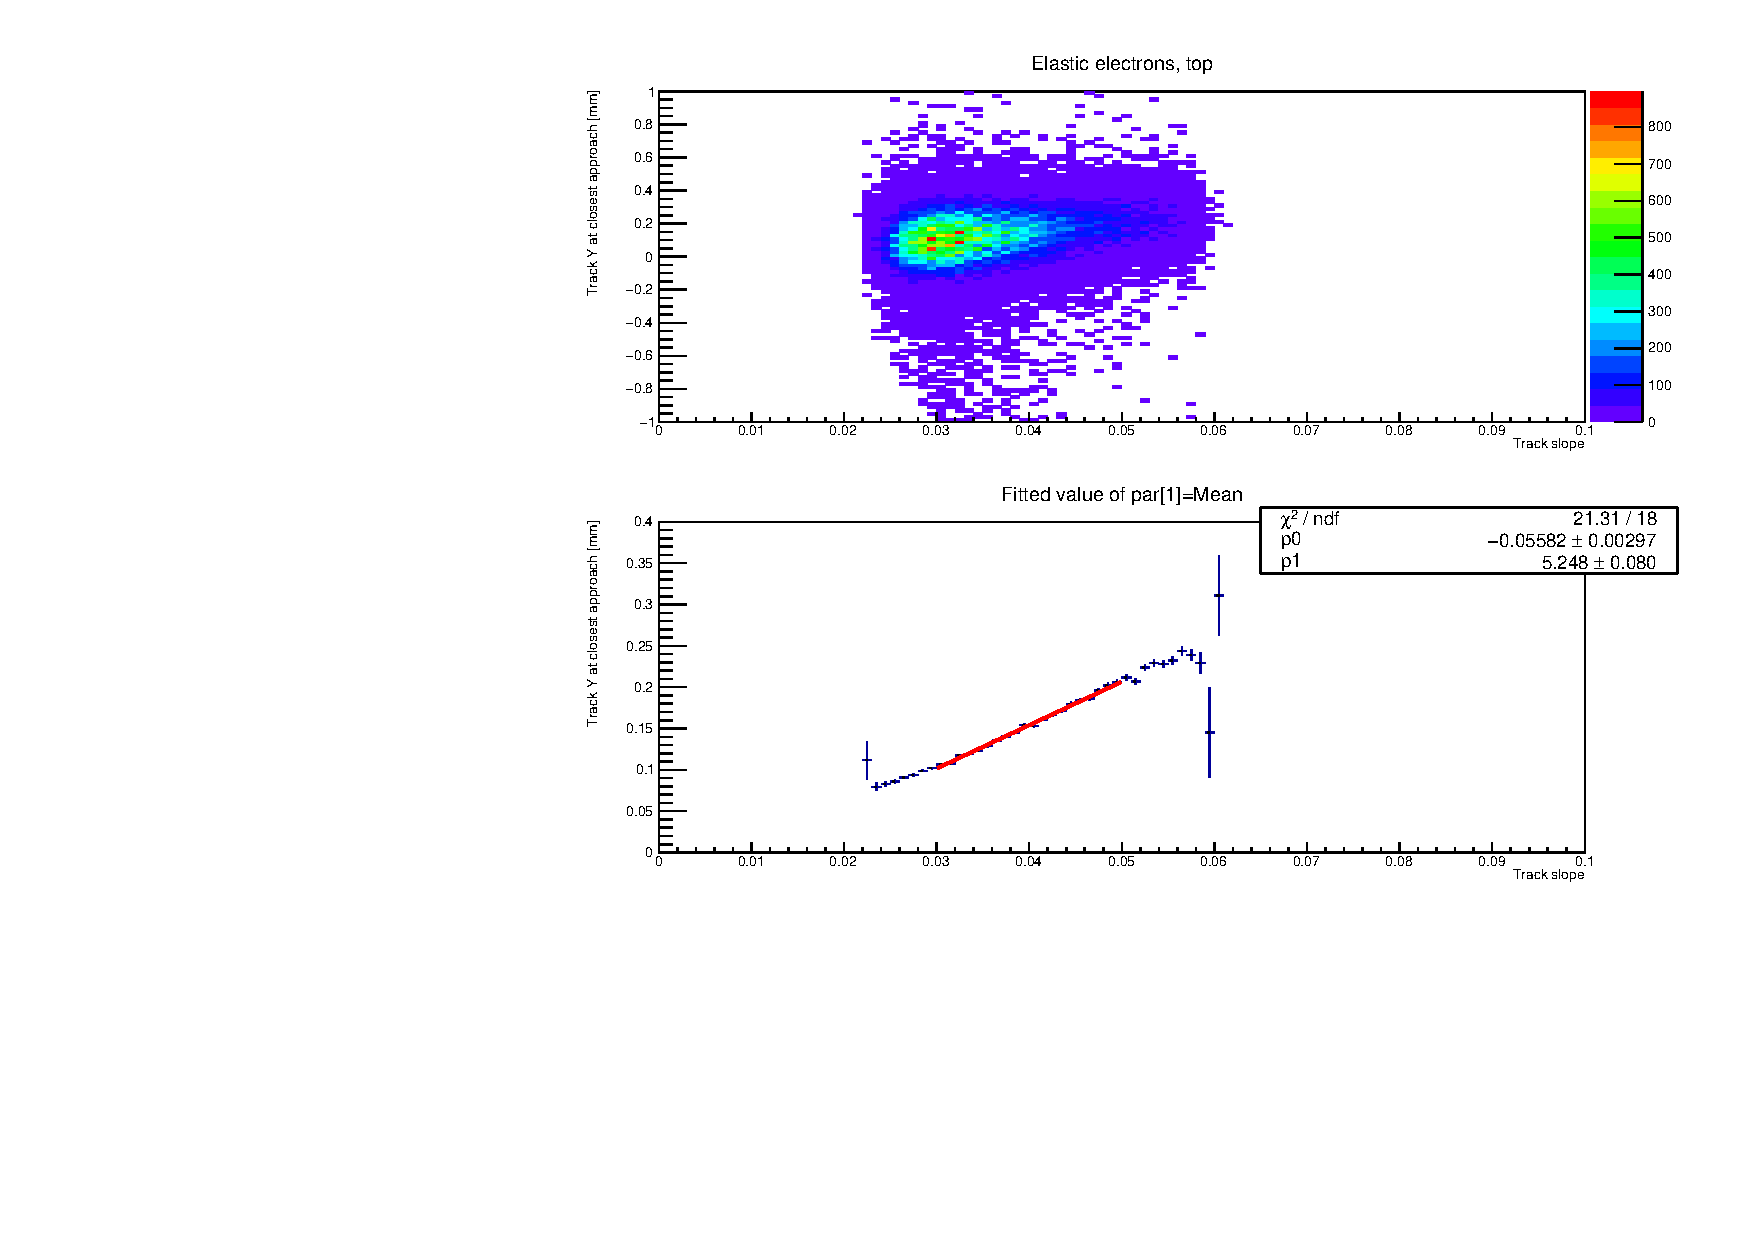
\includegraphics[width=0.6\textwidth,page=1,angle=-90]{recon/figs/fee_angles}
\end{center}
    \caption{
        Top: track slope and $y$ at closest approach, for elastically scattered electrons in the top half of the detector.
        The stripes are the result of single-strip hits in the first layer of the tracker.
        Bottom: each point is the center of a Gaussian fit to a vertical slice of the top histogram.
        The linear fit to the points produces estimates of $y_{beamspot}$ and $z_{target}$.
    }
    \label{fig:feeangles}
\end{figure}

Global alignment corrections are chosen to bring the fitted values of $y_{beamspot}$ close to 0 for both halves of the detector: essentially, the two halves are moved vertically to bring their beamspot measurements into agreement.
The fitted values of $z_{target}$ are consistent with $z_{target}=-5$ mm on both top and bottom.
This could mean that the whole SVT is shifted by $+5$ mm relative to its nominal position (highly unlikely) or that the target is shifted by $-5$ mm (possible).
We believe the target is at $-5$ mm relative to its nominal position, and therefore choose not to apply global alignment corrections to move the SVT by $+5$ mm and bring $z_{target}$ to 0.

The track extrapolation in the X-Z plane is used similarly to find global alignment corrections that bring $x_{beamspot}$ to 0.

\subsection{M{\o}ller Electrons}
\label{sec:mollers}

M{\o}ller scattering events can be identified in the data as $e^-e^-$ pairs with momentum sum equal to the beam momentum.

Because the final state is fully reconstructed, the momentum sum should point in the beam direction.
This is useful for monitoring the beam direction, but it is difficult to use this as a constraint on the global alignment because both halves of the SVT contribute to the measurement of the momentum sum.
Fortunately, the two-body kinematics of M{\o}ller scattering is sufficiently constrained that each electron on its own can provide a constraint, which applies independently to each half of the SVT.

For each electron, there is a strict relation between the energy $E$ and the angle from the beam axis $\theta$.
To lowest order in the electron mass $m_e$, this relation is identical to Compton scattering:
\begin{equation}
    m_e c^2 \left(\frac{1}{E} - \frac{1}{E_{beam}}\right) = (1-\cos{\theta})
    \label{eq:moller_etheta}
\end{equation}

This means that all M{\o}ller electrons with a known energy will have the same angle from the beam axis.
The electron energy is well-measured, since the track curvature has been calibrated using elastic scatters.
Selecting M{\o}ller electrons with energies in a narrow band, as in Figure \ref{fig:mollerangles}, and extrapolating these tracks back to the target, results in a narrow ring of track angles centered at the beam direction.

\begin{figure}[ht]
\begin{center}
    \includegraphics[width=0.6\textwidth,page=2,angle=-90]{recon/figs/mollerplots}
\end{center}
    \caption{
        Angles of M{\o}ller electrons (extrapolated to the target, and relative to the nominal beam direction) in the top half of the detector, in a narrow energy band centered at 400 MeV.
        Equation \ref{eq:moller_etheta} predicts that M{\o}ller electrons at this energy should be emitted at 39.8 milliradians from the beam axis.
    }
    \label{fig:mollerangles}
\end{figure}

Global alignment corrections are used to shift the track angles and center the ring around the nominal beam direction.
Even though only a section of the full ring is captured in the HPS acceptance, there is enough of an arc to determine the horizontal position of the center, and the vertical position of the center can be determined using the radius of the ring (known from Equation \ref{eq:moller_etheta}).

\section{\texorpdfstring{$e^+e^-$}{e+e-} Selection Cuts}
\label{sec:event_selection}
After reconstruction, all possible $e^+e^-$ pairs in the event are tested against a set of cuts.
There is no explicit requirement that the electron and positron be the pair of particles that caused the trigger.
There is also no fiducial requirement, since the inner edge of the detector acceptance is key for sensitivity to low-mass heavy photons.
The base selection is intended to remove accidental coincidences from the pair sample; the pair sample should contain only events where the electron and positron originate in the same interaction.

The ``pairs-1'' trigger is the HPS physics trigger, described in Section \ref{sec:trigger_cuts}.
It is tuned to accept $e^+e^-$ pairs, and is the overwhelming majority of the event rate (16.6 kHz out of 19 kHz).

The electron and positron are required to be in opposite halves of the detector: this cut is implemented as a requirement that the $y$-coordinates of the two clusters have opposite signs.
The trigger requires a top-bottom coincidence, so repeating the requirement as an event selection cut does not reduce the efficiency.
This cut eliminates any possibility of confusion in the track or cluster reconstruction, since the hits from the electron and positron are guaranteed to be well separated.
%A heavy photon can have enough transverse momentum that both decay products land in the same half of the detector, but the rate is low.

Track-cluster matching is important for two reasons: the cluster time resolution is better than the track time resolution, and track-cluster matching eliminates many misreconstructed tracks.
Two checks are done on the quality of the track-cluster matching for both particles.
First, a cut is made on the $\chi^2$ of the track-cluster match; this is a requirement on the distance between the cluster position and the track extrapolation to the ECal.
Second, a cut is made on the track-cluster time difference.
Since the track and cluster times are referenced differently (the track time is relative to the trigger time, and the cluster time is relative to the start of the ECal readout window), a constant offset of 43 ns is subtracted.

Three more simple cleanup cuts are applied.
A loose track quality cut is applied on the $\chi^2$ of each GBL fit; this is only meant to reject very poor track fits.
Elastically scattered electrons with $p(e^-)\approx E_{beam}$ are the main pileup background in the tracker, and are rejected with a maximum momentum requirement on electrons.
A momentum sum cut rejects pairs with a momentum sum too far in excess of $E_{beam}$; this further reduces the rate of random coincidences with elastically scattered electrons.

The last cleanup cut is a cut on the cluster time difference.
This selects time coincidences.
The track time difference could be used similarly, but the cluster time resolution is better.

Finally, a ``radiative cut'' is applied for heavy photon analyses.
This is a minimum requirement on the momentum sum, at $0.8E_{beam}$.
As shown in Section \ref{sec:signal_kinematics}, most heavy photons and radiative tridents are produced with energy near $E_{beam}$; the radiative cut keeps most of these and rejects the Bethe-Heitler tridents that dominate at low momentum.

\begin{table}[ht]
    \begin{center}
        \begin{tabular}{lc}   
            \hline \hline
            Trigger type & ``pairs-1'' trigger \\
            Run and event quality & see Section \ref{sec:luminosity} \\
            Top-bottom requirement & $\sign(y_{cl}(e^-))\neq\sign(y_{cl}(e^-))$ \\
            Track-cluster matching (position) & $\chi^2_{match}<10$ \\
            Track-cluster matching (time) & $|t_{cl}-t_{trk}-43|<4$ ns \\
            Track quality & $\chi^2_{trk}<50$ \\
            Elastics cut & $p(e^-)<0.75E_{beam}$ \\
            Momentum sum cut & $p_{tot}(e^+e^-)<1.15E_{beam}$ \\
            Cluster time coincidence & $|t_{cl}(e^-)-t_{cl}(e^+)|<2$ ns \\
            Radiative cut & $p_{tot}(e^+e^-)>0.8E_{beam}$ \\
            \hline \hline
        \end{tabular}
        \caption{Base pair selection cuts for HPS. The effect of these cuts is shown in Figure \ref{fig:basecut_performance}.}
        \label{tab:basic_cuts} 
    \end{center}
\end{table}

\subsection{Tuning Cuts}
\label{sec:tuning_basecuts}
The cuts are tuned on the data, using the cluster time difference to separate ``good'' and ``bad'' events.
Pairs with large cluster time difference ($|t_{cl}(e^-)-t_{cl}(e^+)|>3$ ns) are accidental coincidences; pairs with small cluster time difference ($|t_{cl}(e^-)-t_{cl}(e^+)|<1$ ns) are dominated by true time coincidences.
An effective cut should reject pairs with large cluster time difference, and not pairs with small cluster time difference.

Figure \ref{fig:basecut_performance} shows the effect of the cuts on the distribution of cluster time differences.
This distribution is the sum of the distributions of true coincidences and random coincidences.
The distribution of true coincidences is a single peak with shape determined by the time resolution, and the distribution of random coincidences is the sum of multiple peaks spaced by the 2 ns beam period, with a slowly varying envelope shaped by the efficiencies of the trigger and track reconstruction.
If (as is the case for all cuts shown in the figure) a cut is not directly sensitive to the cluster time difference, and yet suppresses the outer peaks more than the central peak, it must be rejecting random coincidences.
%Each cut rejects more of the out-of-time events than the in-time events.
%Since the cluster time coincidence cut is the only cut that uses the cluster time difference, this implies that the fraction of accidental coincidences in the central peak decreases

The cluster time coincidence cut is applied after the other cuts, and selects only the central peak.
The rate of random coincidences contaminating the central peak can be estimated from the outer peaks: the fraction of random coincidences after the event selection cuts is roughly 1.5\%.

\begin{figure}[ht]
\begin{center}
    \includegraphics[width=0.6\textwidth,page=2,angle=-90]{recon/figs/basecutplots}
\end{center}
    \caption{Cumulative effect of the different pair selection cuts on pair-1 events passing the top-bottom requirement and radiative cuts.
    The ratio of out-of-time to in-time events (outer peaks to central peak) decreases as cuts are applied (going from the black to the magenta distributions).
    }
    \label{fig:basecut_performance}
\end{figure}

\section{Run Quality, Event Quality, and Data Normalization}
\label{sec:luminosity}
All the data used in the analysis should have the same detector conditions and efficiencies: this is ensured by appropriate selections of runs and events.
The HPS data is divided into runs, which are roughly two hours each unless interrupted by DAQ problems.
All ``golden runs'' included in this analysis have the same configuration for the HPS setup: the tungsten target with design thickness of 0.125\% $X_0$, nominal beam current of 50 nA, the trigger cuts listed in Section \ref{sec:trigger_cuts}, and the SVT position at nominal (layer 1 silicon at 0.5 mm from the beam).

A more fine-grained run quality selection is necessary because even a golden run can include substantial amounts of data that were recorded without the detector being in the desired configuration: a good-quality run can have periods of poor-quality data.
The most common situation is a beam trip.
According to the procedures that were followed by shift workers in the 2015 run, the high-voltage bias to the SVT sensors was lowered when the beam was lost, and bias was only restored after the beam returned.
Furthermore, if the trip was determined to be caused by the halo counter FSD (see Section \ref{sec:beam_quality}), the SVT would be moved out to 1.5 mm from the beam, and only moved back in after the beam returned.
The result is that the SVT would not be in its normal configuration after beam restoration: the bias would be low, and the SVT position might be away from nominal.
Between beam restoration and the restoration of SVT bias and position, data would be recorded but it would not be reconstructable, since at low bias the SVT would not see hits, and at a position away from nominal the SVT alignment would not be correct.

The SVT bias and position history are recorded in a database, and the database is used to find the time intervals when the SVT was in its nominal configuration.
These time ranges are then used to select events with good run quality.

There are additional effects in the SVT that can affect event quality, and can be identified on an event-by-event basis.
The SVT DAQ can enter an error state during a run, which affects all data for the rest of the run for a single sensor; the error state is flagged in each event, so these events are easy to reject.
Roughly 40\% of the data used in this analysis was recorded before the correct setting for the APV25 latency was found; with the incorrect setting, if an event occurs too late relative to the APV25 clock, the SVT hits will not pass the data reduction threshold.
This affects 1/3 of the events in these runs, and the events are identified and rejected based on their trigger timestamps.
Finally, a small fraction (3.5\%) of events in every run have elevated noise in the SVT because the APV25 pipelines were being filled as the APV25 was outputting the digital header for a previous event.
This effect is called ``burst-mode noise'' after the APV25 feature that allows a trigger to be received while a previous event is being read out.
Events with burst-mode noise are identified by counting the number of isolated (no neighboring strips with hits) low-amplitude hits: most normal events have no such hits, and the noisy events have many (tens to hundreds), so this analysis rejects events with 3 or more isolated low-amplitude hits.


Since the expected rate of heavy photons can be normalized to the data, a precise measurement of the integrated luminosity is not critical to the analysis.
Normalizing the data to the integrated luminosity is still essential for understanding the detector efficiencies and comparing the data to the cross sections of known processes.
In order for the integrated luminosity to be useful, it should be corrected for the run and event quality selections.

The luminosity is the product of the beam current, target thickness, and experiment livetime.
The beam current is measured by a Faraday cup, as described in Section \ref{sec:beamline_hallb}.
The target thickness is taken from measurements made during target assembly.
The experiment livetime is the product of the trigger livetime and the SVT DAQ efficiencies (latency and burst-mode noise) explained above.

Section \ref{sec:trigger} explains the two measurements of trigger livetime.
One, from the Faraday cup, measures the fraction of the integrated beam charge which was accumulated with the DAQ live.
The other, from the pulser trigger, measures the fraction of time for which the DAQ was live.
The Faraday cup is more precise, both because it accounts correctly for fluctuations in beam current, and because it has less statistical uncertainty (the Faraday cup scaler rate is roughly 45 kHz at 50 nA, much higher than the 100 Hz frequency of the pulser trigger).
However, the pulser livetime is recorded more frequently (every second, as compared to every 4-5 seconds), and this makes it easier to integrate the luminosity over the run quality time ranges.
A comparison of the Faraday cup and pulser livetimes shows agreement at the 1\% level or better, so the pulser livetime is acceptable.

The luminosity is integrated over the time ranges identified (as explained above) for good SVT bias, good SVT position, and SVT DAQ error status.
The resulting integrated luminosity is appropriate for comparisons with Monte Carlo samples: it assumes an always-on beam, a detector always in its nominal state, and a DAQ that always takes good data.

According to this procedure, the total integrated luminosity for data recorded in the 2015 run with the SVT at 0.5 mm is 1166 nb$^{-1}$.
The unblinded fraction of this data is a total of 119 nb$^{-1}$.

\section{Rate Comparison with Monte Carlo}
\label{sec:rates}

\label{sec:tri_mc}
Simulated samples of all types of $e^+e^-$ pair events of interest (tridents, heavy photons, and wide-angle bremsstrahlung) are generated using MadGraph/MadEvent version 4 \cite{alwall_madgraph/madevent_2007}.
Beam backgrounds, such as elastically scattered electrons, that are created in the target and create pileup in the detector, are simulated using EGS5 \cite{hirayama_egs5_2005} and Geant4 \cite{agostinelli_geant4simulation_2003}.
Particle interactions in the HPS detector are fully simulated using SLIC \cite{graf_simulator_2006}.
The HPS readout and trigger are simulated using software based on the org.lcsim software toolkit \cite{graf_org.lcsim:_2011}.

The trident processes (radiative and Bethe-Heitler tridents, as described in Section \ref{sec:physics_backgrounds}) are simulated using MadGraph/MadEvent.
One generator, called the ``full-diagram'' generator, incorporates all of the trident diagrams and their interference terms, and thus simulates (to lowest order) the combined rate of all $e^-Z\to e^+e^-e^-Z$.
%Both ``full-diagram'' and radiative tridents are simulated using MadGraph/MadEvent.
%The generator for full-diagram tridents includes radiative tridents, Bethe-Heitler tridents, and the interference terms.
Since radiative tridents are important for normalizing the heavy photon rate, a separate generator is used to generate radiative tridents on their own.
The heavy photon Monte Carlo generator, and the use of the radiative trident Monte Carlo sample, is explained in Chapter \ref{sec:vertexing}.

Wide-angle bremsstrahlung conversions (WABs) are the other important source of $e^+e^-$ pairs; as explained in Section \ref{sec:physics_backgrounds}, the primary electron and the positron from the pair conversion can fake an $e^+e^-$ pair.
MadGraph/MadEvent is used to produce $e^-\gamma$ events because it handles the angle correlations and the momentum transfer to the nucleus correctly.
The photon pair conversion is simulated in EGS5 (if in the target) or Geant4 (if in the SVT).

Ignoring random coincidences (as shown in Section \ref{sec:tuning_basecuts}, they are a small contribution), we believe the pair events in the data are fully simulated by the sum of the full-diagram trident and WAB generators.
Figure \ref{fig:esum_allpairs_uncorr} shows the momentum sum (the magnitude of the total pair momentum) for data and the two Monte Carlo samples.
If the Monte Carlo samples fully describe the data, the data histogram should match the sum of the Monte Carlo histograms, but it does not.
Instead the rate in data undershoots the rate in Monte Carlo at every value of the momentum sum.

\begin{figure}[ht]
\begin{center}
    \includegraphics[width=0.6\textwidth,page=2,angle=-90]{recon/figs/wabratioplots}
\end{center}
    \caption{Momentum sum $p(e^+e^-)$ for data (black), Monte Carlo samples of tridents (red) and wide-angle bremsstrahlung conversions (blue), and the sum of the red and blue histograms (magenta).
    All histograms are normalized to integrated luminosity such that the sum of all bins for a histogram equals the total cross-section in nanobarns.
    If Monte Carlo completely describes data, black and magenta histograms should match.
    %Note the agreement at high momentum sum (not remarkable, since it is by construction).
    }
    \label{fig:esum_allpairs_uncorr}
\end{figure}

Preliminary studies suggest that there is a significant inefficiency in the track reconstruction that is not reflected in the Monte Carlo.
Since the heavy photon analysis only uses pairs with momentum sum above $0.8\times E_{beam}$, it is most important to characterize the problem in that region of phase space.

We make the assumption that the inefficiency uniformly affects all high-momentum pairs.
%To make the data and Monte Carlo rates agree for $p_{tot}(e^+e^-)>0.8\times E_{beam}$, the necessary difference between data and Monte Carlo efficiencies for high-momentum pairs is 0.65.
Scaling the data histogram by $1/0.65$, as in Figure \ref{fig:esum_allpairs}, forces the data and Monte Carlo rates to agree at high momentum sum; this is equivalent to assuming that there is an 65\% efficiency factor that is present in data but not in Monte Carlo.
Since the rates at lower momentum sums do not agree, either the efficiency effect is momentum-dependent, or there is another explanation (such as a problem with the MadGraph/MadEvent generator) for the discrepancy at low momentum sums.
In either case we must justify assuming uniform inefficiency at high momentum sum, when the behavior at lower momentum sum is clearly different.
We must show that after scaling the data, the data and Monte Carlo agree at high momentum sum --- the rates agree by construction, but other comparisons should also agree.

\begin{figure}[ht]
\begin{center}
    \includegraphics[width=0.6\textwidth,page=36,angle=-90]{recon/figs/wabratioplots}
\end{center}
    \caption{Same histograms as Figure \ref{fig:esum_allpairs_uncorr}, except that data is multiplied by 1/0.65 to account for the estimated level of detector inefficiency at high momentum.
    If Monte Carlo completely describes data, black and magenta histograms should match.
    Note the agreement at high momentum sum (not remarkable, since it is by construction).
    }
    \label{fig:esum_allpairs}
\end{figure}

One such comparison is to check the relative rates of tridents and WABs.
Tridents and WABs have significantly different kinematics, and might be expected to be affected differently by a momentum-dependent inefficiency.
Since the MadGraph/MadEvent generators are different for the two Monte Carlo samples, a problem affecting one generator would change the relative rates of the two samples.
Several variables can be used to separate tridents from WABs.

One variable identifying WABs is the absence of a hit in layer 1 of the SVT for the positron track.
A trident positron should always (aside from detector inefficiencies) have a layer 1 hit, since the positron is created in the target and the angular acceptances are roughly the same for all layers.
WAB conversions often occur in layer 1 (or later), and the positron track will not have a layer 1 hit unless the conversion occurs in the upstream sensor of the layer 1 stereo pair.
Figure \ref{fig:esum_l1pos} shows the momentum sum for pairs with and without layer 1 hits on the positron track.
In both, data and Monte Carlo show good agreement at high momentum sum.
This indicates that data and Monte Carlo agree on the relative rates of tridents and WABs; the same efficiency applies to both.
%Roughly speaking, since the upstream sensor of layer 2 is the last place the conversion can happen and still result in a positron track, and the rate of conversions in the target ($\sim 0.125$\% $X_0$) is small compared to the rate of conversions in silicon ($0.35$\% $X_0$ per sensor), 

\begin{figure}[ht]
\begin{center}
    \includegraphics[width=0.35\textwidth,page=38,angle=-90]{recon/figs/wabratioplots}
    \includegraphics[width=0.35\textwidth,page=40,angle=-90]{recon/figs/wabratioplots}
\end{center}
    \caption{Same histograms as Figure \ref{fig:esum_allpairs}, but the left plot requires that the positron track have a layer 1 hit, which rejects most WAB conversions, and the right plot requires that the positron track not have a layer 1 hit, which rejects most tridents.
    Note the continued agreement between data and Monte Carlo at high momentum sum.
    }
    \label{fig:esum_l1pos}
\end{figure}

WABs can also be separated by looking at the positron track's distance of closest approach.
If the pair conversion happens in silicon and not the target, the positron track will not extrapolate to the target, but will instead miss to the side in the X-Z plane.
This can be seen in Figure \ref{fig:pos_d0}, which plots the positron track's distance of closest approach for pairs with high momentum sum: the distribution for trident Monte Carlo events is symmetric around the beam spot, but the distribution for WAB Monte Carlo events is strongly skewed.
Data agrees with the sum of the two Monte Carlo samples, which again supports the conclusion that Monte Carlo describes the data well at high momentum.

\begin{figure}[ht]
\begin{center}
    \includegraphics[width=0.6\textwidth,page=8,angle=-90]{recon/figs/wabratioplots}
\end{center}
    \caption{Distance of closest approach in the X-Z plane for the positron track, only plotting pairs with momentum sum above 0.8 times the beam energy (radiative cut).
    This is centered at 0 (where the beam spot is) if the positron comes from the target, but is usually positive for WAB positrons created downstream of the target.
    }
    \label{fig:pos_d0}
\end{figure}

Finally, WABs can be separated based on the direction of the pair momentum.
Since the WAB positron is created in the pair conversion of a photon, the electron from the pair conversion is created at a similar angle in the Y-Z plane; both are on the same side of the beam plane.
This means the electron from the pair conversion is never part of the $e^+e^-$ pair that passes the selection cuts in Section \ref{sec:event_selection}, and therefore that the positron in a WAB event is always on the same side of the beam plane as the missing electron.
Since the momenta of the two electrons and the positron approximately sum to the beam momentum (the momentum transfer to the nucleus is typically not large), this means that the momentum of the positron is on the opposite side of the beam plane from the total momentum of the $e^+e^-$ pair.
In contrast, radiative tridents have no such correlation, and Bethe-Heitler tridents have the opposite correlation.
Figure \ref{fig:pt_y} plots (for pairs with high momentum sum) the $y$-component of the momentum sum times the sign of the $y$-component of the positron momentum, and shows that this is typically negative for the Monte Carlo WAB sample and positive for the Monte Carlo trident sample.
Again, data agrees with the sum of the two Monte Carlo samples, which again supports the conclusion that Monte Carlo describes the data well at high momentum.

\begin{figure}[ht]
\begin{center}
    \includegraphics[width=0.6\textwidth,page=10,angle=-90]{recon/figs/wabratioplots}
\end{center}
    \caption{$p(e^+e^-)_y\sign(p(e^+)_y)$, only plotting pairs with momentum sum above 0.8 times the beam energy (radiative cut).
    This is positive if the pair momentum points in the same direction as the positron.
    }
    \label{fig:pt_y}
\end{figure}

We conclude that after the radiative cut, the Monte Carlo samples describe the data well, except that the rate in data is 0.65 times the rate expected from Monte Carlo.
